\hspace*{12pt}Los resultados obtenidos para el diagrama Magnitud V-I son los que siguen (Ver Figura \ref{VIdiag}).

	\begin{figure}[!htbp]
		\centering
		\begin{center}
			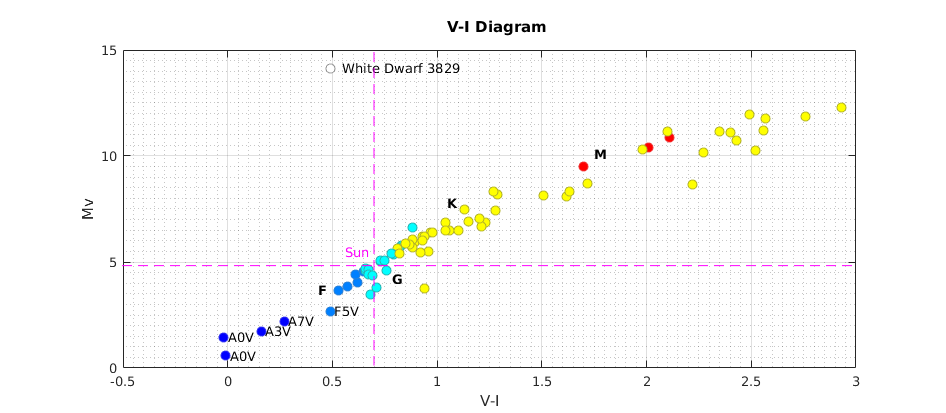
\includegraphics[width=15cm]{Figures/VIdiagram.png}
		\end{center}
		\caption{\footnotesize{En el siguiente diagrama se ha representado la relaci\'{o} entre la magnitud absoluta de cada estrella y su color V-I. Ambas cantidades est\'{a}n representadas en magnitudes.}}
		\label{VIdiag}
		\end{figure}

\hspace*{12pt} Como se puede observar en la Figura \ref{VIdiag} los resultados son muy similares a los obtenidos para el diagrama HR de la Figura \ref{HRdiag} excepto porque las diferencias entre la magnitud de las bandas V e I es mucho mayor (En magnitudes) que la diferencia entre las bandas B y V. Esto es debido a la forma de cuerpo negro que tiene la emisi\'{o}n estelar, en la cual una vez pasado el pico de emisi\'{o}n, situado cerca del V generalizando mucho, la curva del cuerpo negro cae de manera m\'{a}s abrupta que lo que sub\'{i}a antes del pico.